\documentclass[11pt,a4paper]{ctexart}
\usepackage[top=1in,bottom=1in,left=1.25in,right=1.25in]{geometry}
\usepackage{graphicx}
\usepackage{tikz}
\usepackage{times,bitmetr}
\usepackage{algorithmic}
\usepackage{algorithm}
\usepackage{array}
\usepackage{mdwmath}
\usepackage{mdwtab}
\usepackage{amsmath}
\usepackage{amsfonts}
\usepackage{amssymb}
%\usepackage{anysize}
\usepackage{subfigure}
\usepackage{pifont}
\usepackage{color}
\usepackage{float}
\usepackage{soul}
\usepackage{tabu}
\bibliographystyle{IEEEtran}



\title{Research Report Three}
\author{Xinpeng Hong
	\thanks{The author acknowledges the support of wavelab in
		making this project a reality}\\
	\\\\
}



% Change to the current month of the series
\reportmonth{October 17}
% Change to the current year of the series
\reportyear{2019}
% Change to the TR number that you obtained from the
% UWEETR web pages when you initially created a new
% TR number. Only provide the last 4 digits here, the year
% goes in the \reportyear{} field above.
\reportnumber{0003}



\begin{document}
\makecover
\maketitle
	

\section{SeqGAN论文实验}
\subsection{实验结果}
\noindent 首先比较序列生成性能如下表;负对数似然收敛的训练阶段如下图。\\\\
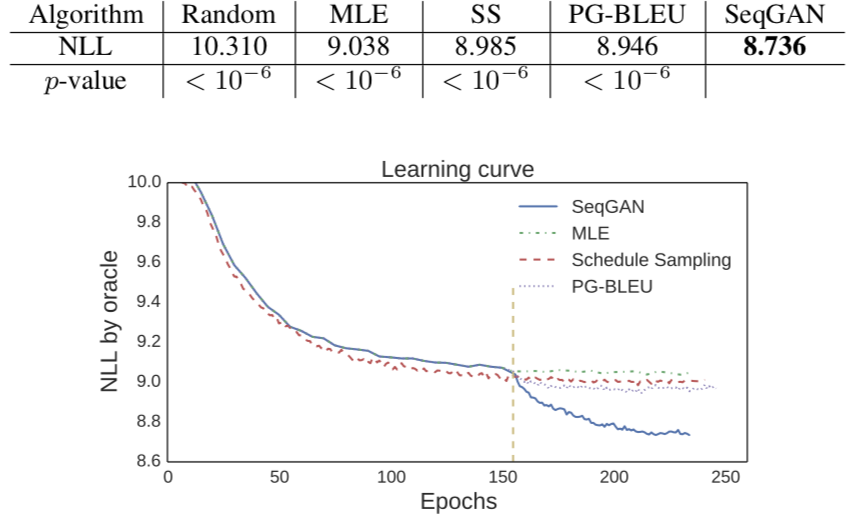
\includegraphics[scale=1]{1.png}\\\\\\\\\\\\\\
\indent \indent \indent \indent 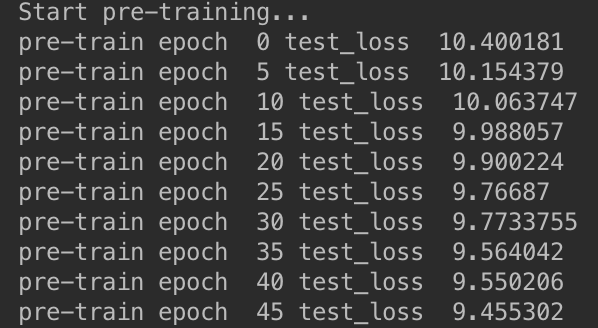
\includegraphics[scale=1]{2.png}\\
SeqGAN的NLL最后趋于约8.736。\\
不同训练策略下SeqGAN的负对数似然收敛性能如下。\\
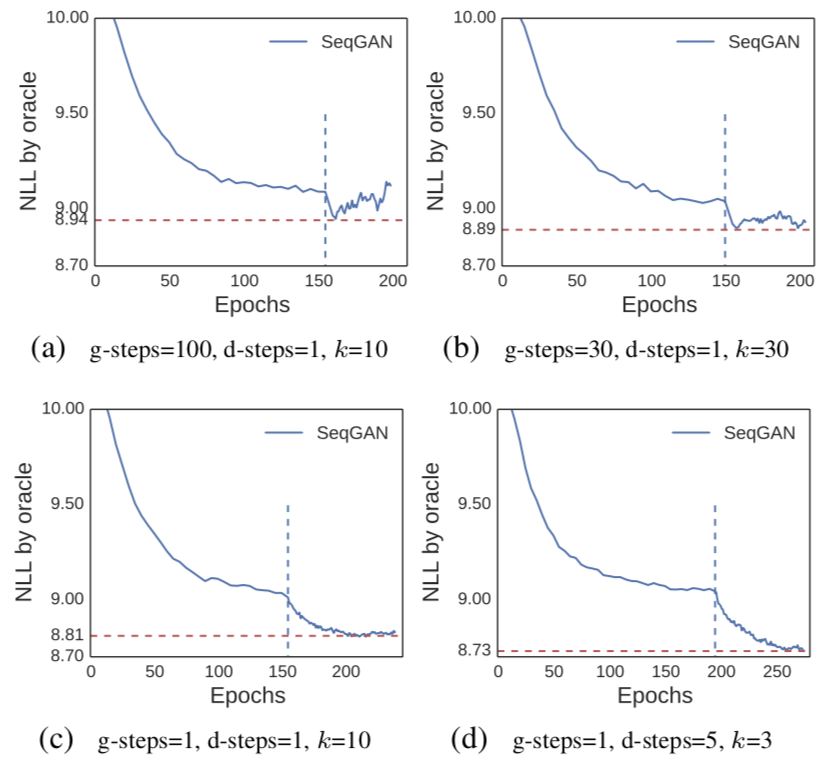
\includegraphics[scale=1]{3.png}\\
我发现SeqGAN的稳定性取决于训练策略,更具体地说,即算法中的g步、d步和参数k对SeqGAN的收敛性和性能有很大的影响。\\\\\\
在图(a)中,g-steps远远大于d-steps和epoch number k。该策略收敛速度快,但随着生成器的快速改进,判别器不能得到充分的训练,从而逐渐产生误导信号。\\
在图(b)中,随着判别器训练时间的增加,不稳定的训练过程得到了缓解。\\
在图(c)中,我们只训练一个epoch,g-step等于d-step,SeqGAN能稳定学习。上述三种训练策略中的d-step都设置为1,这意味着我们只生成一组与给定数据集数目相同的负样本,然后针对不同的k来训练判别器。实际上我们可以利用潜在的无限数量的负样本来改进判别器,我们可以将固定的正样本与不同的负样本结合起来以得到多个训练集。\\
从图(d)中可以看出,该方法可以提高训练生成器的整体性能,具有良好的稳定性,因为识别器会显示更多的负样本,这将为训练生成器提供更全面的指导。
\section{相关论文阅读}
\subsection{Online Anomaly Detection on the Webscope S5 Dataset: A Comparative Study}
\noindent 这篇论文主要说的是,目前的异常检测算法大多遵循将异常归类为与预测结果有显著偏差的一般思路,他们对几种在线异常检测算法在大型Yahoo Webscope S5异常基准上进行了比较研究,发现一种相对简单的在线回归异常检测器(SORAD)与其它异常检测器相比是成功的。他们的长期目标是通过其他各种简单的在线自适应算法来扩展SORAD,然后形成一个异常检测算法的集合。\\
利用滑动窗口方法生成特征,离线回归算法(Offline-RAD)进行异常检测,在线估计正态分布的均值和方差,Online-RAD能规避一些Offline-RAD的弊端,并把SORAD用在Webscope S5 Dataset上做实验。
\subsection{Towards Experienced Anomaly Detector through Reinforcement Learning}
\noindent 这篇论文主要提出了一种时间序列异常检测的方法,该检测器不考虑异常模式的潜在机制,避免了在特定场景下为获得良好的异常检测性能而进行阈值设置的繁琐工作,随着异常检测经验的增长而不断演进。该异常检测器本质上是由递归神经网络(RNN)驱动,采用增强学习(RL)方法实现自学习过程。他们的初步实验证明了该检测器在网络时间序列异常检测中的应用前景。\\
RNN采用的是LSTM,RL采用带记忆回放的Q-learning方法。使用滑动窗口方法将每个时间序列转换为一组多维数据实例。Q-learning中的动作是a∈{0,1},其中0表示无异常,否则为1。另一方面,Q-learning中的状态被设计成数据的串联和之前执行动作的固定记录。为了提高模型训练的过程,采用了二叉树策略,在训练的经验集合中分别加入对前状态s执行不同动作0和1所产生的s ' 0和s ' 1两种状态。换句话说,在我们的训练中,a state s会增加两条记录,即⟨s, a= 0, r0, s′0⟩和⟨s, a= 1, r1, s′1⟩。r0和r1是在s状态下执行不同动作所获得的奖励,根据数据集的标签设计奖励函数。\\\\\\\subsection{DeepAnT: A Deep Learning Approach for Unsupervised Anomaly Detection in Time Series}
\noindent 这篇论文提出了一种新的基于深度学习的时间序列数据异常检测方法(DeepAnT),与学习异常的异常检测方法相比,DeepAnT使用未标记的数据来捕获和学习用于预测时间序列的正常行为的数据分布。DeepAnT由时间序列预测器和异常检测器两个模块组成,时间序列预测器模块使用深度卷积神经网络(CNN)来预测在定义的视界上的下一个时间戳,此模块采用时间序列窗口(用作上下文),并尝试预测下一个时间戳,然后将预测值传递给异常检测模块,该模块负责将相应的时间戳标记为正常或异常。\\
在基于深度学习的方法中,需要大量数据来训练模型。而在DeepAnT中,由于CNN的有效参数共享,模型可以在相对较小的数据集上训练,同时获得良好的泛化能力。由于DeepAnT中的异常检测是无监督的,因此在生成模型时不依赖于异常标签,因此,这种方法可以直接应用于真实的场景。
\subsection{总结}
\noindent 以上三篇论文都可以用做我们的baseline。
\section{交大报告IDEA}
\noindent 正在尝试将SeqGAN的思想运用在异常检测以证明可行,目前还在尝试阶段,如果可行,下一步是复现CLSTM+GAN,比较实验效果。\\
一个困惑是每次尝试的实验时间非常长,不知道是否有改善的方法?
	
\end{document}